\documentclass[notes,11pt, aspectratio=169]{beamer}

\usepackage{pgfpages}
% These slides also contain speaker notes. You can print just the slides,
% just the notes, or both, depending on the setting below. Comment out the want
% you want.
\setbeameroption{hide notes} % Only slide
%\setbeameroption{show only notes} % Only notes
%\setbeameroption{show notes on second screen=right} % Both

\usepackage{helvet}
\usepackage[default]{lato}
\usepackage{array}

\usepackage[backend=biber,style=authoryear,
sorting=ynt,citestyle=authoryear]{biblatex}
\addbibresource{Paper/papercitations.bib}

\usepackage{tikz}
\usepackage{verbatim}
\setbeamertemplate{note page}{\pagecolor{yellow!5}\insertnote}
\usetikzlibrary{positioning}
\usetikzlibrary{snakes}
\usetikzlibrary{calc}
\usetikzlibrary{arrows}
\usetikzlibrary{decorations.markings}
\usetikzlibrary{shapes.misc}
\usetikzlibrary{matrix,shapes,arrows,fit,tikzmark}
\usepackage{amsmath}
\usepackage{mathpazo}
\usepackage{hyperref}
\usepackage{lipsum}
\usepackage{multimedia}
\usepackage{graphicx}
\usepackage{multirow}
\usepackage{graphicx}
\usepackage{dcolumn}
\usepackage{bbm}
\newcolumntype{d}[0]{D{.}{.}{5}}
\usepackage{subfigure}
\usepackage{import}

\usepackage{changepage}
\usepackage{appendixnumberbeamer}
\newcommand{\beginbackup}{
   \newcounter{framenumbervorappendix}
   \setcounter{framenumbervorappendix}{\value{framenumber}}
   \setbeamertemplate{footline}
   {
     \leavevmode%
     \hline
     box{%
       \begin{beamercolorbox}[wd=\paperwidth,ht=2.25ex,dp=1ex,right]{footlinecolor}%
%         \insertframenumber  \hspace*{2ex} 
       \end{beamercolorbox}}%
     \vskip0pt%
   }
 }
\newcommand{\backupend}{
   \addtocounter{framenumbervorappendix}{-\value{framenumber}}
   \addtocounter{framenumber}{\value{framenumbervorappendix}} 
}

\setbeamertemplate{blocks}[rounded]
\setbeamercolor{block title}{bg=purple, fg=white}
\setbeamercolor{block body}{bg=purple!10}

\usepackage{graphicx}
\usepackage[space]{grffile}
\usepackage{booktabs}

% These are my colors -- there are many like them, but these ones are mine.
\definecolor{sage}{RGB}{102,153,102}
\definecolor{yellow}{RGB}{255,173,1}
\definecolor{purple}{RGB}{153,102,153}

% colors for diagrams
\definecolor{diagramtan}{RGB}{225,190,106}
\definecolor{diagramteal}{RGB}{64, 176, 166}
\definecolor{diagrampurple}{RGB}{170, 131, 239}
\definecolor{diagramred}{RGB}{146, 79, 79}


\hypersetup{
  colorlinks=false,
  linkbordercolor = {white},
  linkcolor = {sage}
}

\newcommand{\btVFill}{\vskip0pt plus 1filll}


%% I use a beige off white for my background
\definecolor{MyBackground}{RGB}{255,253,218}

%% Uncomment this if you want to change the background color to something else
%\setbeamercolor{background canvas}{bg=MyBackground}

%% Change the bg color to adjust your transition slide background color!
\newenvironment{transitionframe}{
  \setbeamercolor{background canvas}{bg=white}
  \begin{frame}}{
    \end{frame}
}

\setbeamercolor{frametitle}{fg=black}
\setbeamercolor{title}{fg=black}
\setbeamertemplate{footline}[frame number]
\setbeamertemplate{navigation symbols}{} 
\setbeamertemplate{itemize items}{$\rightarrow$}
\setbeamercolor{itemize item}{fg=sage}
\setbeamercolor{itemize subitem}{fg=sage}
\setbeamercolor{enumerate item}{fg=sage}
\setbeamercolor{enumerate subitem}{fg=sage}
\setbeamercolor{button}{bg=sage,fg=white}



% If you like road maps, rather than having clutter at the top, have a roadmap show up at the end of each section 
% (and after your introduction)
% Uncomment this is if you want the roadmap!
\AtBeginSection[]
{
   \begin{frame}
       \frametitle{Roadmap of Talk}
       \tableofcontents[currentsection]
   \end{frame}
}
\setbeamercolor{section in toc}{fg=sage}
\setbeamercolor{subsection in toc}{fg=sage}
\setbeamersize{text margin left=1em,text margin right=1em} 

\newenvironment{wideitemize}{\itemize\addtolength{\itemsep}{10pt}}{\enditemize}

\usepackage{environ}
\NewEnviron{videoframe}[1]{
  \begin{frame}
    \vspace{-8pt}
    \begin{columns}[onlytextwidth, T] % align columns
      \begin{column}{.58\textwidth}
        \begin{minipage}[t][\textheight][t]
          {\dimexpr\textwidth}
          \vspace{8pt}
          \hspace{4pt} {\Large \sc \textcolor{blue}{#1}}
          \vspace{8pt}
          
          \BODY
        \end{minipage}
      \end{column}%
      \hfill%
      \begin{column}{.42\textwidth}
        \colorbox{green!20}{\begin{minipage}[t][1.2\textheight][t]
            {\dimexpr\textwidth}
            Face goes here
          \end{minipage}}
      \end{column}%
    \end{columns}
  \end{frame}
}

\title[]{\textcolor{sage}{Does Hospital Leadership Matter? \newline
Evidence from Pay-for-Performance}}

\author[]{Hanna Glenn \newline
2024-2025 Job Market Candidate}
\date{}


\begin{document}

%%% TIKZ STUFF
\tikzset{   
        every picture/.style={remember picture,baseline},
        every node/.style={anchor=base,align=center,outer sep=1.5pt},
        every path/.style={thick},
        }
\newcommand\marktopleft[1]{%
    \tikz[overlay,remember picture] 
        \node (marker-#1-a) at (-.3em,.3em) {};%
}
\newcommand\markbottomright[2]{%
    \tikz[overlay,remember picture] 
        \node (marker-#1-b) at (0em,0em) {};%
}
\tikzstyle{every picture}+=[remember picture] 
\tikzstyle{mybox} =[draw=black, very thick, rectangle, inner sep=10pt, inner ysep=20pt]
\tikzstyle{fancytitle} =[draw=black,fill=red, text=white]
%%%% END TIKZ STUFF

% Title Slide
\begin{frame}
\begin{center}
    \huge
    \vspace{7mm}
    Hanna Glenn
    \vspace{2mm}
    
    \large
    2024-2025 Job Market Candidate

    \btVFill

    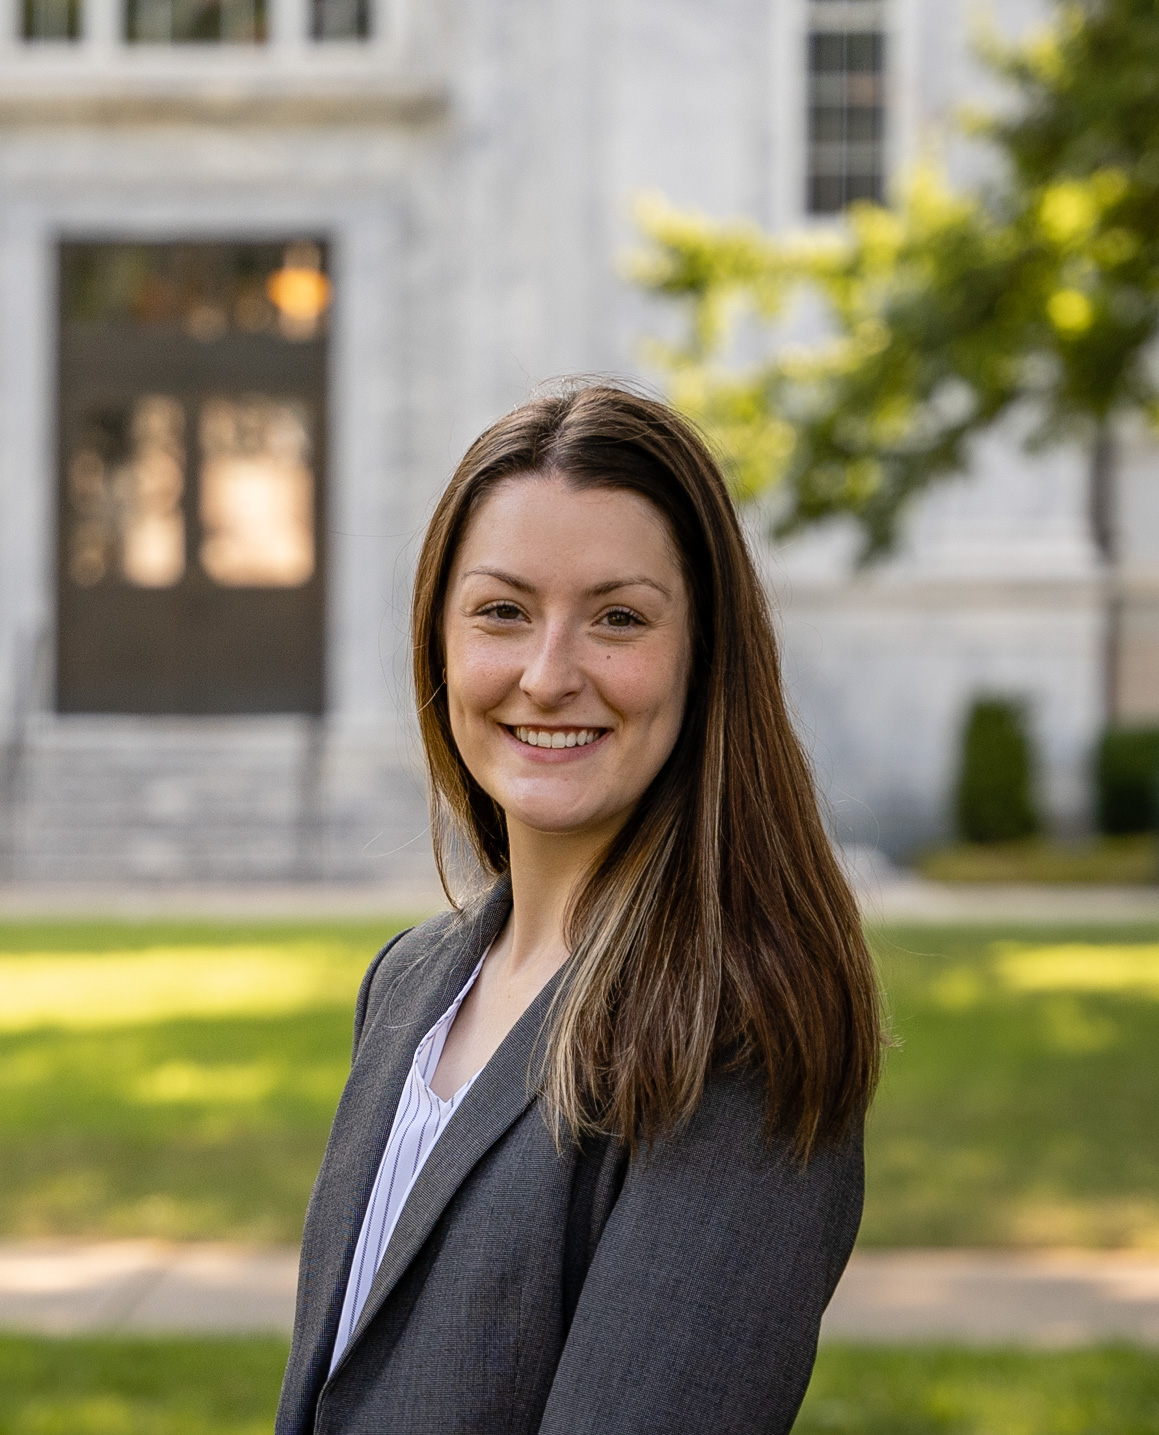
\includegraphics[scale=.4]{Graphics/HannaGlenn_headshot.jpg}
    
\end{center}
\end{frame}

\begin{frame}{}
    \begin{tikzpicture}
        % First image in the top-left
        \node[anchor=north west] at (0, 4) {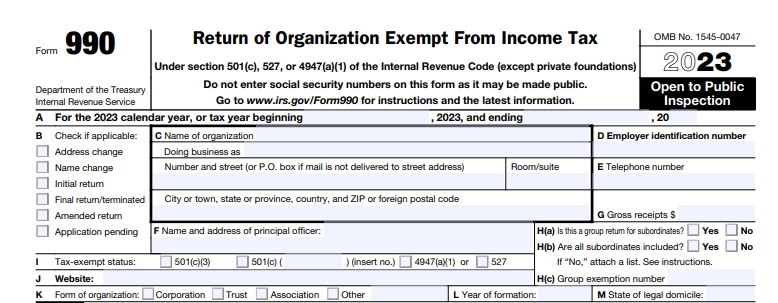
\includegraphics[width=0.7\textwidth]{Graphics/990_snip_frontpage.PNG}};
        % Second image in the middle
        \node[anchor=north west] (img2) at (2.5, 1.5) {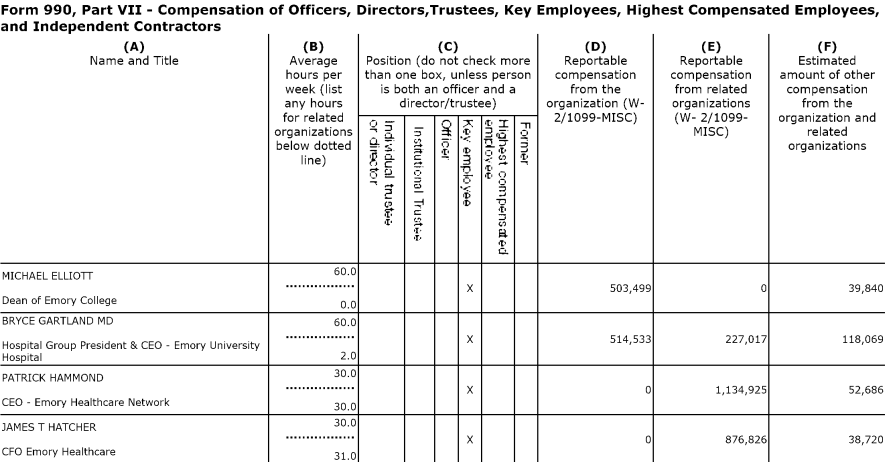
\includegraphics[width=0.75\textwidth]{Graphics/Screenshot 2024-10-03 160258.png}};
        \draw[line width=1mm, sage] (img2.north west) rectangle (img2.south east);
    \end{tikzpicture}
\end{frame}

\begin{frame}{Readmission Rates}
\centering
    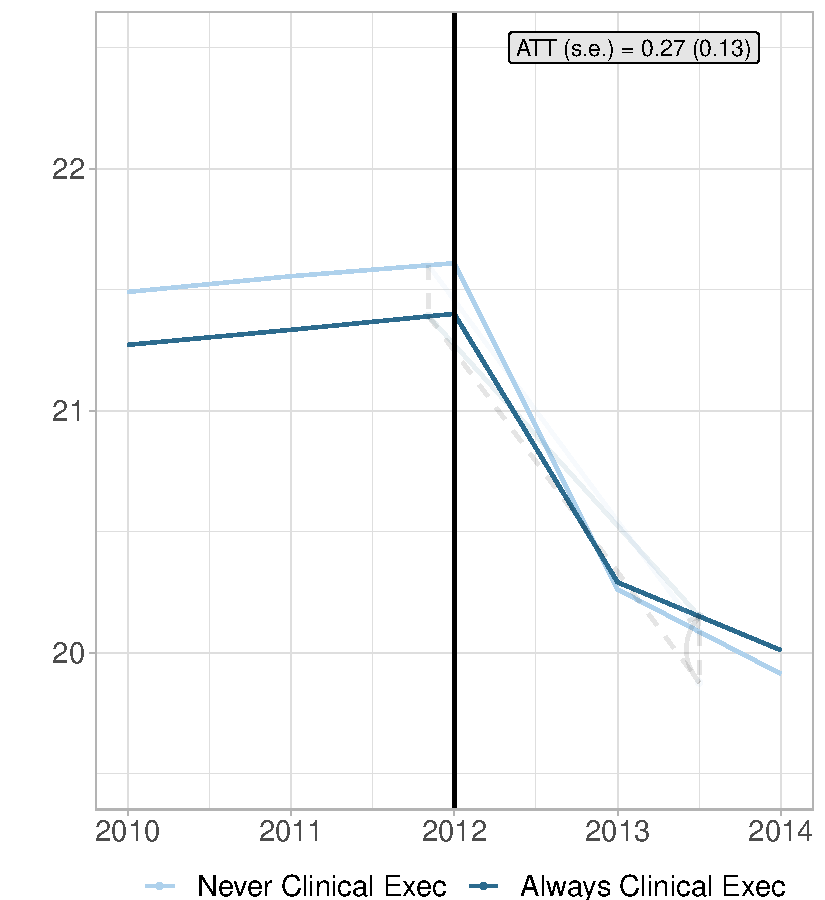
\includegraphics[width=.45\textwidth]{Objects/read_md_nomd_synth_graph.pdf}
\end{frame}

\begin{frame}{}
        \centering
    \begin{tikzpicture}
        % First image (top-left)
        \node[anchor=north west] (img1) at (0, 4) {
\includegraphics[width=0.5\textwidth]{Graphics/news1.png}};
        \draw[line width=.5mm, sage] (img1.north west) rectangle (img1.south east);
        
        % Second image (slightly down and right of the first image)
        \node[anchor=north west] (img2) at (6, 2.5) {
\includegraphics[width=0.55\textwidth]{Graphics/news2.png}};
        \draw[line width=.5mm, sage] (img2.north west) rectangle (img2.south east);
        
        % Third image (further down and left)
        \node[anchor=north west] (img3) at (.25, .75) {
\includegraphics[width=0.55\textwidth]{Graphics/news3.png}};
        \draw[line width=.5mm, sage] (img3.north west) rectangle (img3.south east);
        
        % Fourth image (bottom-right)
        \node[anchor=north west] (img4) at (3, -1.5) {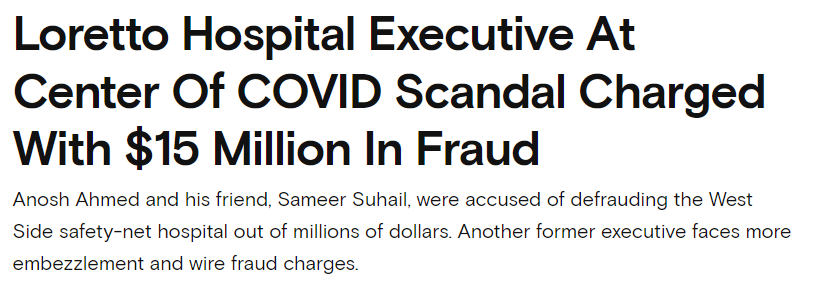
\includegraphics[width=0.45\textwidth]{Graphics/news4.png}};
        \draw[line width=.5mm, sage] (img4.north west) rectangle (img4.south east);
    \end{tikzpicture}
\end{frame}



\end{document}